%\newpage
\section{Auswertung}
    \subsection{Bestimmung der Untergrundrate}
    \label{sec:untergrund}
        In einem Zeitraum von $T = \SI{327256}{s}$ wurden $N_{\text{Start}} = 6543685$ Startsignale und $N_{\text{Stopp}} = 25257$
        Stoppsignale aufgenommen. Damit ergibt sich eine durchschnittliche Rate von:
        \begin{equation*}
            r = \frac{N_{\text{Start}}}{T} = \frac{6543685}{327256} \approx 20,00 \, \frac{\text{Myonen}}{\text{s}}
        \end{equation*}
        Die Wahrscheinlichkeit, dass genau ein weiteres Myon ($k = 1$) in der Suchzeit $T_\text{S} = \SI{10}{\micro s}$ nach dem Eintreffen eines vorherigen Myons ein Signal erzeugt, ist poissonverteilt und damit:
        \begin{align*}
            p(k) &= \frac{(T_{\text{S}} \cdot r)^k}{k!} \exp\left(-T_{\text{S}} \cdot r\right) \\[10pt]
            p(1) &= T_{\text{S}} r \cdot \exp\left(-T_{\text{S}}  r\right) \approx \SI{0,02000}{\%}
        \end{align*}
        Der Untergrund setzt sich aus diesen während einer angefangenen Suchzeit ankommenden Myonen zusammen. Also ist die Anzahl dieser fehlerhaften Signale gegeben durch:
        \begin{equation*}
            N_{\text{fehl}} = p(1) \cdot N_{\text{Start}} \approx 1308
        \end{equation*}
        Für jeden der 225 besetzten Kanäle (gesamt 512 Kanäle) im MCA wäre der Untergrund somit:
        \begin{equation*}
            u_{\text{theo}} \approx 5,81
        \end{equation*}

    \subsection{Justierung der Verzörgerungsleitungen}
        Die Signale aus den Photomultipliern sollten möglichst zeitgleich an der Koinzidenz ankommen. Das heißt, dass die Anzahl der Signale, die die Koinzidenz durchlässt steigt je kleiner der zeitliche Abstand zwischen den beiden ankommenden Signalen ist. 
        Da die Pulsdauer des Ausgangssignales am Diskriminator auf \SI{10}{\nano \second} normiert ist, kann innerhalb dieser Pulsdauer das Signal des anderen Diskriminators an der Koinzidenz ankommen und kann als gleichzeitig betrachtet werden.
        Deshalb ist ein Plateau in \autoref{fig:Verzoergerung} zu sehen, wenn die Counts gegen die Zeitdifferenz auftragen werden.
        
        \begin{figure}[h]
            \centering
            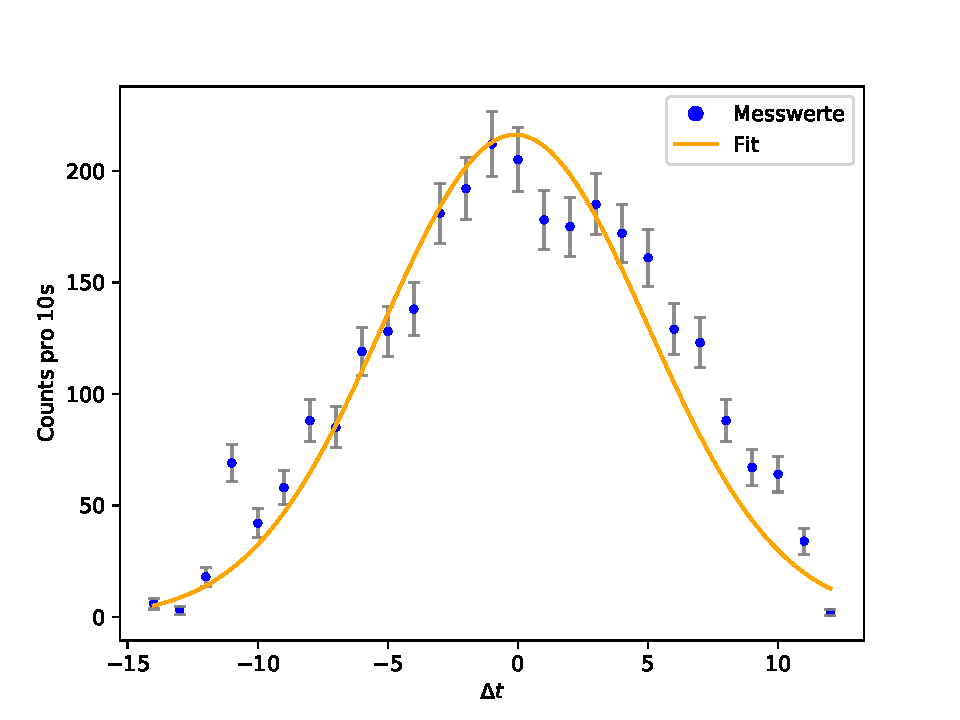
\includegraphics[width = 0.75\textwidth]{plots/Verzoergerung.pdf}
            \caption{Die an der Koinzidenz gemessenen Counts/10s sind gegen die Zeitdifferenz zwischen den beiden Verzörgerungsleitungen aufgetragen. Die zugehörigen Fehler sind als Fehlerbalken dargestellt. Die Halbwertsbreite wird durch die gestrichelten Linien dargestellt.}
            \label{fig:Verzoergerung}
        \end{figure}

        \FloatBarrier

        Da es sich bei Zählraten um poissonverteilte Größen handelt, kann für die Fehler der Counts $N = \sqrt{N}$ geschrieben werden. Diese sind in Form von Fehlerbalken in \autoref{fig:Verzoergerung} eingetragen.

        Es wird die Plateau-Funktion
        \begin{equation*}
            f(x) = a \exp\left(-\left(\frac{x - x_0}{\sigma}\right)^{2 n}\right)
        \end{equation*}
        mit dem Paramater $n = 2$ an die Messwerte gefittet.
        Für ein höheres $n$ würde die Funktion ein stärker ausgeprägtes Plateau aufweisen, doch sie würde sich nicht mehr so gut an die gemessenen Werte fitten lassen. Das Plateau wäre zu weit von den oberen Werten entfernt.
        Die sich durch die Ausgleichsrechnung ergebenden Parameter
        \begin{align*}
            a &= 170,63 \pm 8,53 \\
            x_0 &= (-0,036 \pm 0,219) \, \text{ns} \\
            \sigma &= (9,03 \pm 0,22) \, \text{ns}
        \end{align*}

        Aus der angepassten Funktion lässt sich die Halbwertsbreite zu $T_{\text{FWHM}} = \SI{16,4}{\nano \second}$ bestimmen.

        Im Nachfolgenden wurde die Stelle der maximalen Counts als Nullpunkt gewählt und alle darauffolgenden Schritte wurden mit den entsprechend eingestellten Verzörgerungsleitungen durchgeführt.

    \subsection{Kalibration des TAC-MCA}
        Das TAC gibt zu einem gemessenen Zeitintervall proportionale Spannungsamplitude an den MCA weiter, welche dann ihrer Größe nach in Kanäle geordnet werden. Um den Proportionalitätsfaktor zwischen den Amplituden und den Zeitintervallen zu bestimmen werden 11 Pulsabstände von $0.3\;\mu$s bis $9.9\;\mu$s an einem Doppelimpulsgenerator eingestellt und gegen die Kanäle im MCA aufgetragen. Dadurch kann bestimmt werden welchem Kanal welcher Zeitabstand zugeordnet ist, bzw. welcher Propotionalitätsfaktor zwischen den Zeitabständen und den Kanälen am MCA herrscht.

        \begin{figure}[h]
            \centering
            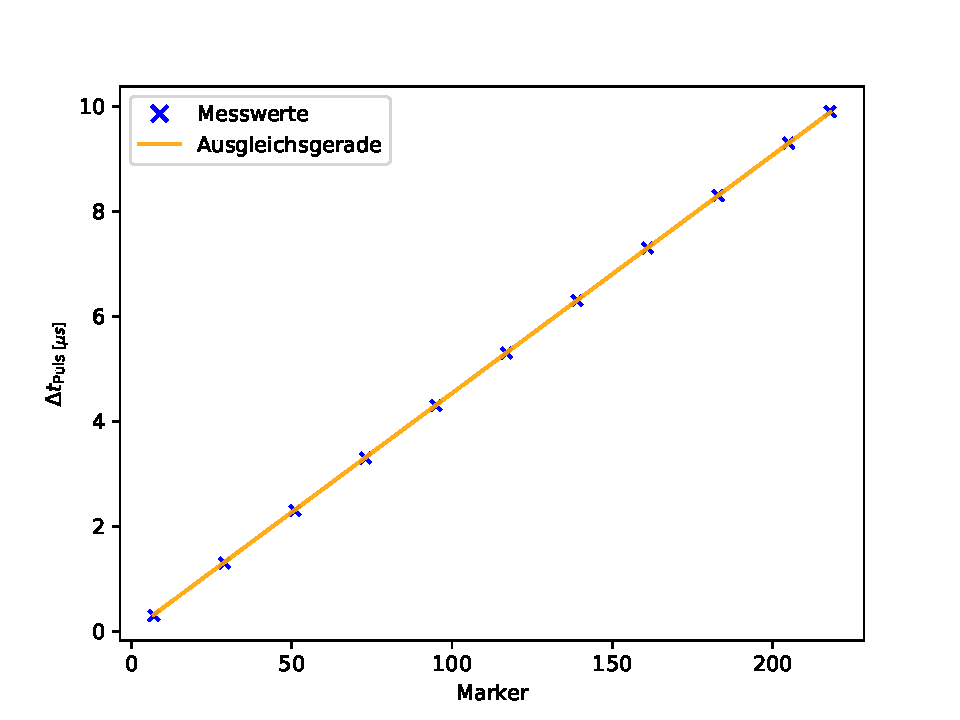
\includegraphics[width = 0.75\textwidth]{plots/Marker_Faktor.pdf}
            \caption{Das eingestellte Zeitintervall zwischen den Pulsen am Doppelimpulsgenerator ist gegen die Kanäle des MCA aufgetragen. Dabei wird eine Ausgleichsgerade an die Messwerte gelegt.}
            \label{fig:Marker_Faktor}
        \end{figure}

        \FloatBarrier

        An die Messwerte wird eine lineare Ausgleichsgerade der folgenden Form gelegt
        \begin{equation*}
            f(x) = m \cdot x
        \end{equation*}
        mit der Steigung:
        \begin{equation*}
            m = (0,045348 \pm 0,000024) \, \mu\text{s}
        \end{equation*}
    
    \newpage
    \subsection{Bestimmung der Lebenszeit}
        \begin{figure}[h]
            \centering
            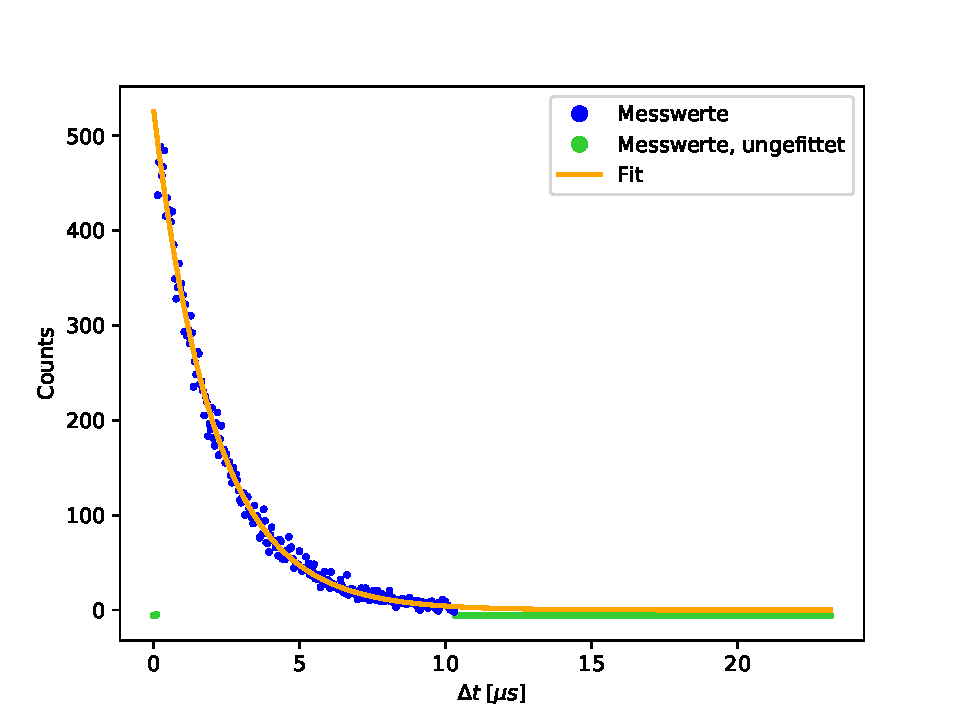
\includegraphics[width = 0.8\textwidth]{plots/Lebenszeit.pdf}
            \caption{Die über 4 Tage aufgenommenen Counts sind gegen die Zeitintervalle vom Start bis zum Stopp der jeweiligen Messung aufgetragen. Aufgrund der Einschränkung durch das gewählte Messintervall werden die grün markierten Messpunkte nicht beachtet.}
            \label{fig:Lebenszeit}
        \end{figure}

        \FloatBarrier

        Über einen Zeitraum von ca. 90,9 Stunden wurden 25257 Myonen-Zerfälle aufgenommen. In \autoref{fig:Lebenszeit} ist wie zu erwarten ein exponentieller Verlauf der Lebenszeit zu erkennen. Zur Bestimmung der Zerfallskonstante $\lambda$ aus dem Zerfallsgesetz \eqref{eqn:Zerfallsgesetz} wird eine Exponentialfunktion an die Messwerte gefittet, von denen der in \autoref{sec:untergrund} theoretisch berechnete Untergrund abgezogen wurde:
        \begin{equation*}
            f(x) = A \cdot \exp\left(-\lambda x\right)
        \end{equation*}
        Als Parameter ergeben sich:
        \begin{align*}
            \lambda &= (0,4827 \pm 0,0043) \, \mu\text{s}^{-1}
        \end{align*}
        Der zuvor berechnete Untergrund von $u_{\text{theo}} \approx 5,81$ ist in der Messunsicherheit enthalten.

        Mit $\lambda$ ergibt sich eine mittlere Myonenlebensdauer von
        \begin{equation*}
            \tau_{\mu} = \frac{1}{\lambda} = (2,072 \pm 0,0118) \, \mu\text{s}
        \end{equation*}
        mit einer relativen Messabweichung vom Theoriewert $\tau_{\text{theo}} \approx 2,197 \, \mu$s \cite{zyla_review_2020} von:
        \begin{equation*}
            a_{\tau} = \frac{\tau_{\mu} - \tau_{\text{theo}}}{\tau_{\text{theo}}} \approx 5,7 \;\%    
        \end{equation*}


















































